\documentclass[a4paper,10pt]{scrartcl}
\usepackage[utf8x]{inputenc}
\usepackage[T1]{fontenc}
\usepackage{amsmath,amsfonts,amssymb,amscd,amsthm,xspace}
\usepackage[english]{babel}
\usepackage{listingsutf8}
\usepackage{color}
\usepackage{geometry}
\usepackage{graphicx}
\usepackage{multicol}
\usepackage{pst-tree}

\geometry{a4paper, left=2cm,right=2cm,top=2cm,bottom=2cm}

\newcommand{\Authors}{Robert Fels - Rollnumber: EX2014005}
\title{Principles of Embedded System Design  - Assignment 1}
\author{\Authors}
\date{\today}

\newcommand{\changefont}[3]{\fontfamily{#1} \fontseries{#2} \fontshape{#3} \selectfont}

\renewcommand{\thesection}{Task \arabic{section}:}
\renewcommand{\theenumi}{(\alph{enumi})}
\renewcommand{\theenumii}{(\roman{enumii}}

\definecolor{lgray}{gray}{0.95}
\definecolor{purple}{rgb}{0.498,0,0.3333}
\definecolor{identifier}{rgb}{0,0,0.1}
\definecolor{string}{rgb}{0.192,0,1}
\definecolor{comment}{rgb}{0.25,0.5,0.37}

\pagestyle{myheadings}
\oddsidemargin\oddsidemargin
\markright{\Authors}

\lstset{
	tabsize=4, 
	frame=tlrb, 
	basicstyle=\footnotesize\changefont{pcr}{m}{n},
	breaklines=true,
	numbers=left,
	emphstyle=\textit, 
	language=Java,
	keywordstyle=\color{purple}\textbf, 
	identifierstyle=\color{identifier},
	stringstyle=\color{string},
	backgroundcolor=\color{lgray},
	showstringspaces=false,
	commentstyle=\color{comment},
	extendedchars=true,
	inputencoding=utf8/latin1
}
\psset{nodesep=2pt,levelsep=2em,treesep=2em}

\begin{document}

\maketitle

\section{Number of switching functions with n variables}

Let  $ f(x_{1}, x_{2}, .. , x_{n}) \rightarrow X$ be a switching function where $X \in \{0,1\}$ and $n$ the number of Variables. Hence you can choose for each of the $n$ variables either the value $0$ or $1$ what means that you can have $$\underbrace{2*2*2* .. * 2}_\text{n - times}= 2^{n}$$ different possible variable configurations. The result of the switching function $ f(x_{1}, x_{2}, .. , x_{n})$ can be either $0$ or $1$ for each of the $2^{n}$ too. As a result there are $$\underbrace{2 * 2 * 2 * .. * 2}_{2^{n}\text{- times}} = 2 ^{2^{n}}$$ possible switching functions when all the $n$ variables are involved in the result of the switching functions. \newline \newline
Assume that not all the variables have to be involved in the result of the switching functions. The amount of switching functions will increase because the configurations of $2^{n}$ variables and less, e.g. $2^{n-1}$ variables has to be considered. In consequence there will be $$ 2 ^{2^{n}} + 2 ^{2^{n -1}} + 2 ^{2^{n -2}} + .. + 2 = \sum\limits_{i=0}^n 2 ^{2^{i}}$$ possible switching functions which not necessarily involving all the variables.

\section{Reading exercise: Chapter 1 \& 2 of Wayne Wolf’s book}

\section{Combinational circuit for 4 Bit Divider}

The combinational circuit to divide 2 4-bit numbers is realized with the help of half adders, full adders, multiplexers and OR and NOT symbols. [see Figure \ref{fig:divider}]
\begin{figure}[h!]
\centering
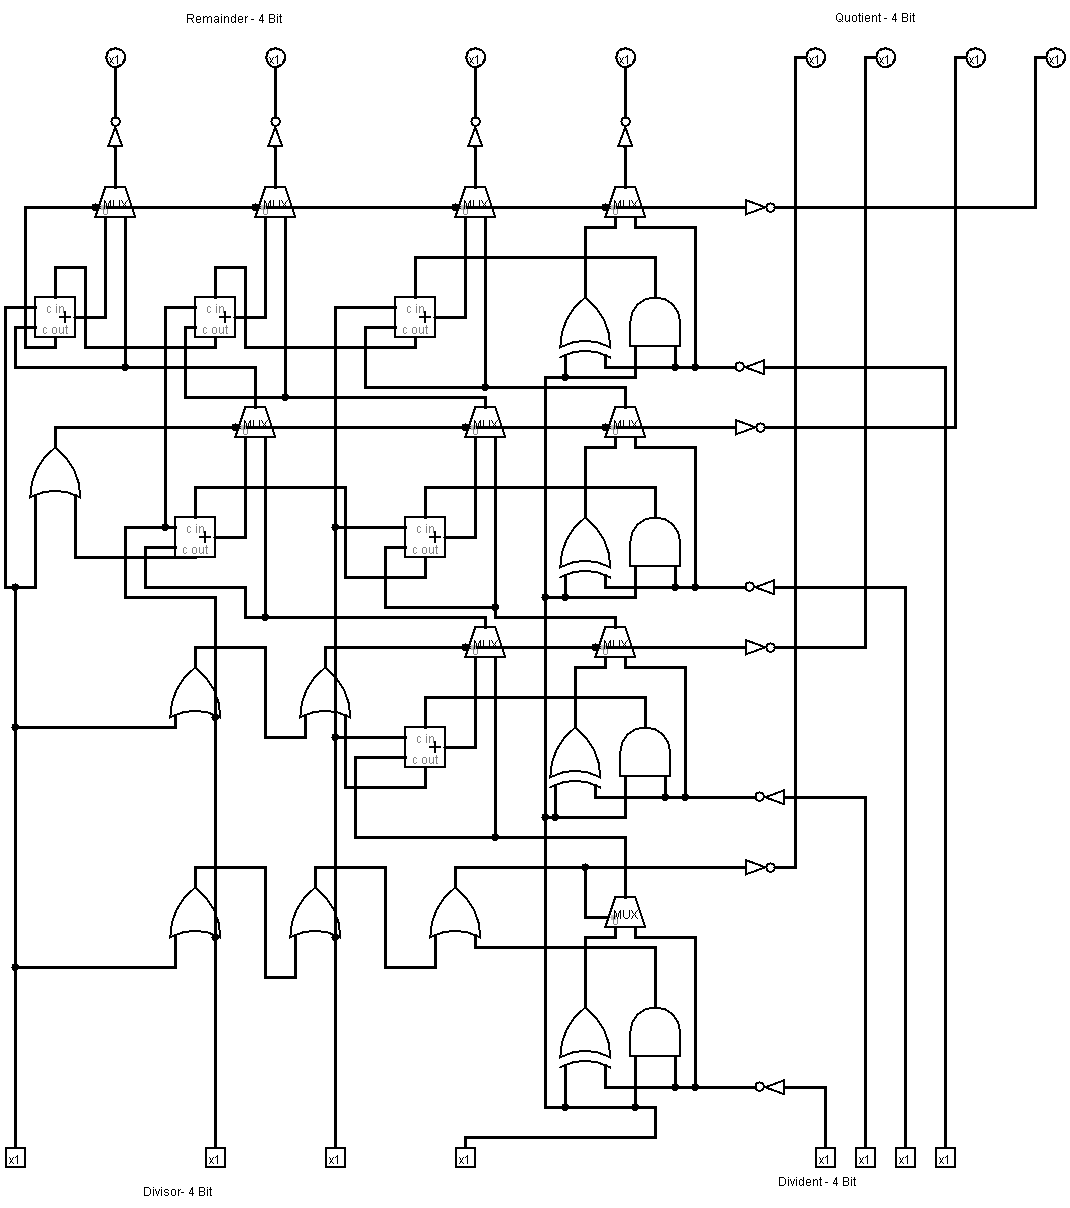
\includegraphics[width=\textwidth]{4BitDivider.png}
\caption{4 Bit Divider}
\label{fig:divider}
\end{figure}

I'll send the file with the divisor circuit and the tool logism to open the file attached to the email. The tool logism doesn't need to be installed, the program will run immediately when opening the logism*.exe on any Windows system.

\newpage
\section{FIR in C using circular buffer}
Please see the code in the attachment.
\section{Calculations of an Embedded System}
We have an embedded system with the following inputs:
\begin{itemize}
\item 16 bit audio, 2 channels at the frequency range 300Hz - 17 KHz
\item 2 cams with 30 fps and 320x240 frame size, each RGB-pixel a resulution of 8 bit
\end{itemize}

\textit{Question:} How much memory is needed to store 1 sec input?
\begin{enumerate}
\item Memory for the 2 cams:

$2 * (30 * (320*240) * 8)$ bit $ =  36864000$ bit $= 4500$  KB per second \newline
Explanation: 2 (cams) * (30 (frames) * 320*240 (pixel) * 8 (bit per pixel) per second

\item Memory for the audio:

$ 17000$ Hz $* 16$ bit $* 2$ (\#channel) $= 544000$ bits per second $=  66.41$ KB per second \newline

\item In Total there will be $(4500 + 66.41)$ KB $= 4566.41$ KB needed to store a second of the input data.
\end{enumerate}

The embedded system is using a 64 coefficient FIR filter for the audio channels and 9 sample median filtering on the images. Each operation takes 1 clock cycle and the memory access need 1 clock cycle too. 


\textit{Question:} The clock speed is 600 MHz. Will the system run in real time? In other words is it possible to do all necessary computations in 1 ms?

\begin{enumerate}
\item Clock speed the 2 cameras are using:

$ 2* (0.03 * 320 * 240) * ( 9 + 9 + 1) = 87552 $ operations per millisecond

Explanation: 2 (cams) (0.03 frames/ms * 320 * 240 pixel) * ( 9 (read all 9 Pixel) + 9 (sort nlog(n)) + 1 (replace middle value) 

\item Clock speed the FIR filter is using:

2 * 9 * 64 * 17 = 19584 operations per millisecond

Explanation: 2 (\#channel) * 9 * 64  (operations in FIR per coefficient) * 17 * 1/ms (frequency)

\item In total the processor supports 600000 operations per millisecond. The FIR and the 2 cameras are using only 87552 + 19584 = 107136 operations per millisecond. Hence the system should be able to run in real time.
\end{enumerate}


\section{C code for finding integer roots of a quadratic equation with 32 bit integer coefficients}
Please see the code in the attachment.

\end{document}